\documentclass[french]{article}
\usepackage{makecell}

\usepackage[utf8]{inputenc} % encode en UTF8

\usepackage[T1]{fontenc}





\usepackage[top=2cm, bottom=2cm, left=3cm, right=3cm]{geometry}
\usepackage{graphicx}
\usepackage{caption}
\usepackage{subcaption}
\usepackage{float}
\graphicspath{ {./photo/} }

%Belles fraction de fration \cfrac
\usepackage{amsmath}

\usepackage{tikz}
\usepackage{circuitikz}
\renewcommand{\contentsname}{Table des matières}
\renewcommand{\listfigurename}{Table des figures}
\renewcommand{\listtablename}{Liste des tableaux}


\parindent=0cm 

\usepackage{listings}             % Include the listings-package

\lstset{language=Matlab}          % Set your language (you can change the language for each code-block optionally)



%\lstdefinestyle{CStyle}{
%	backgroundcolor=\color{backgroundColour},
%	commentstyle=\color{mGreen},
%	keywordstyle=\color{magenta},
%	numberstyle=\tiny\color{mGray},
%	stringstyle=\color{mPurple},
%	basicstyle=\footnotesize,
%	breakatwhitespace=false,
%	breaklines=true,
%	captionpos=b,
%	keepspaces=true,
%	numbers=left,
%	numbersep=5pt,
%	showspaces=false,
%	showstringspaces=false,
%	showtabs=false,
%	tabsize=2,
%	language=C
%}




\newcommand{\HRule}{\rule{\linewidth}{0.5mm}} % Epaisseur des lignes horizontales

\pagestyle{empty}
\newcommand{\myTitle[1]}{
\begin{minipage}{.47\textwidth}
\centering
\begin{flushleft}

\includegraphics[width=0.75\textwidth]{./photo/nantes_universite_logo.png}
\end{flushleft}
\end{minipage}
\begin{minipage}{.47\textwidth}
\centering
\begin{flushright}
\hspace*{1cm} 
\includegraphics[width=0.85\textwidth]{./photo/logo_polytech_nantes}
\end{flushright}
\end{minipage}~\\[1.5cm]

\begin{center}
\vspace*{\stretch{0.3}}
\end{center}

\begin{center}
  \Large
  \vspace*{\stretch{1}}
  \HRule \\[0.2cm]
  \begin{center}
    \huge
    \textbf{#1}\\ %Titre
  \end{center}
  %\textbf{\\ Projet Transversal}\\ %matière
  \HRule \\[1.5cm]
  
%  \vspace*{\stretch{5}}
%  
%  \small
%  \noindent Rédigé par \\
%  \vspace*{\stretch{0.2}}
%  \large
%  \noindent \Redac\\
%  \vspace*{\stretch{0.5}}
 
\end{center}

\vspace*{\stretch{2}}

\begin{center}\large
	\textsc{École Polytech de Nantes}\\
	\textsc{Département Électronique et Technologie du Numérique}
\end{center}

\vspace*{\stretch{5}}

\begin{center}
	\begin{minipage}{0.4\textwidth}
		\begin{flushleft} \large
        	\noindent Rédigé par\\ %\Redac
			Mathis BRIARD \\
			Victor DUFRENE
		\end{flushleft}
	\end{minipage}
	\begin{minipage}{0.4\textwidth}
		\begin{flushright}\large
			Professeur encadrant : \\Olivier PASQUIER
		\end{flushright}
	\end{minipage}
\end{center}
}


\begin{document}
	\myTitle[Rapport d'exécutifs temps-réel \\ - Transfert de messages - ]
	\newpage
	
	\tableofcontents
	\newpage
	\listoffigures
	\listoftables
	\newpage
	
	
	\vspace*{4cm}
	\section*{Résumé}
	L'exécutif temps-réel de systèmes électroniques est une discipline essentielle lorsqu'il s'agit, dans le cadre d'une future carrière d'ingénieur, de réaliser un produit répondant à des contraintes de temps. Et ce domaine est d'autant plus indispensable dans un monde où les systèmes numériques sont de plus en plus complexes et rapides, demandant de réaliser des tâches dans une fenêtre de temps bien déterminé. Ce rapport s'inscrit dans la présentation d'une application affichant l'heure sur un écran.

	
	\newpage
	\pagestyle{plain} % Début de la numérotation des pages
	
	\section{Introduction}
	\subsection{Contextualisation}
	La formation ETN (Électronique et technologies numériques) offerte par l'école polytechnique de l'Université de Nantes propose d'aborder diverses branches de l'électronique, du traitement du signal au systèmes à microprocesseur en passant par l'électronique analogique des hautes-fréquences. Cet ensemble de domaines techniques nécessite des compétences en matière de méthodologie de conception. Ce rapport s'inscrit dans la conception d'un appareil de marquage routier avec la méthode MCSE. La méthode MCSE (Méthode de conception des systèmes électroniques), née à Ireste par l'impulsion de Jean-Paul Calvez, cette méthode a été implantée au sein d'un outil nommée CoFluent rachetée par Intel\mbox{\textregistered } depuis 2011. Cette méthode fait désormais partie de la culture de la formation et constitue l'outil de conception premier de l'ingénieur ETN.\\
	Ce rapport se décompose en diverses parties. Il s'agira dans un premier temps de rappeler le cahier des charges de la conception de cet appareil de marquage routier. Dans un second temps la partie spécification sera traitée et pour finir il s'agira de parler de la conception.\\
	
	
	\subsection{Objectifs}
	Ce rapport vise à retranscrire les résultats du travail pratique réalisé sur les files (transferts) de messages. Les objectifs des manipulations étaient d'utiliser le mécanisme de boîte aux lettres puis d'estimer l'utilisé de l'exclusion mutuelle.
	
	\newpage
	
	\section{Situation}
	
	
	La situation que nous visons à implémenter est une file de message qui permet la communication inter-processus. L'application considérer est celle d'un système qui affiche l'heure dont la structure fonctionnelle est donné à la figure \ref{fig:structure_fontionnelle}.
	
	\begin{figure}[H]
		\centering
		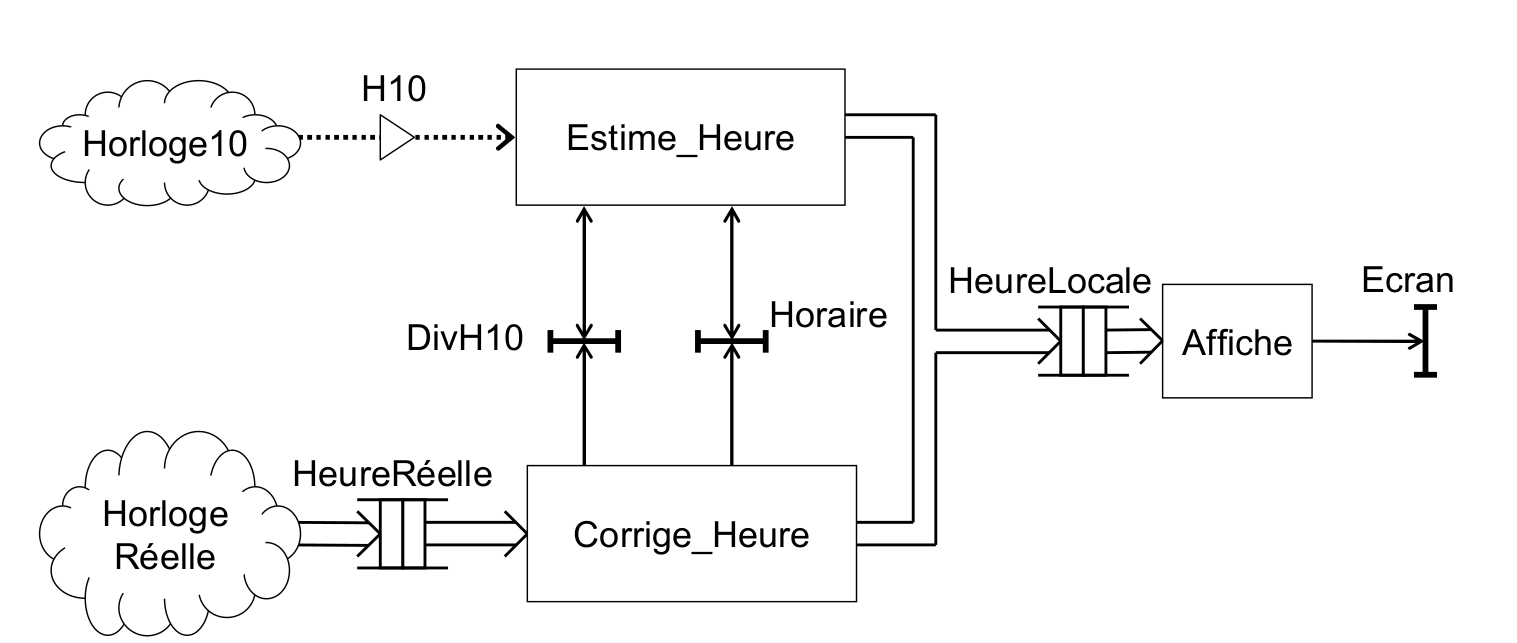
\includegraphics[width=13cm]{photo/situation}
		\caption{Sortie sur la console}
		\label{fig:structure_fontionnelle}
	\end{figure}
	
	L’application consiste à afficher sur Ecran, l’heure (heure, minute, seconde). L’heure
peut être obtenue par estimation à partir d’une horloge à 10Hz (H10) et pour éviter les
dérives, l’heure réelle est reçue par l’intermédiaire de HeureRéelle (heure, minute, seconde).
	Pour information, afin de limiter la longueur des observations, la base de temps de
l’environnement est beaucoup plus rapide que la seconde.
	

	\subsection*{Fonction Estime\_Heure}
	
	
	Action activée sur H10, événement périodique apparaissant 10 fois par seconde. Elle
incrémente la variable DivH10 si elle est inférieure à 9, sinon elle met la variable à 0 et la
variable Horaire est incrémentée d’une seconde. Un message est transmis dans HeureLocale.
	Le message indique que la valeur transmise est une valeur estimée et contient la nouvelle	valeur de Horaire.
	
	\subsection*{Fonction Corrige\_Heure}
	
	Action activée sur HeureRéelle. Elle copie la valeur reçue dans Horaire, met la
variable DivH10 à 0 et transmet un message dans HeureLocale. Le message indique que la
valeur transmise est une valeur réelle et contient la nouvelle valeur de Horaire.
	
	\subsection*{Fonction Affiche}
	
	Cette fonction copie sur Ecran l’heure reçue par l’intermédiaire de HeureLocale en
indiquant s’il s’agit de l’heure estimée ou de l’heure réelle (c’est la seule tâche ou vous
pouvez faire un printf).\\
	
	
	Le réseau de Pétri qui décrit le comportement des fonctions \texttt{Estime\_Heure} et \texttt{Corrige\_Heure} est donné à la figure \ref{fig:reseau_petri} ci-dessous.
	
	
	\begin{figure}[H]
		\centering
		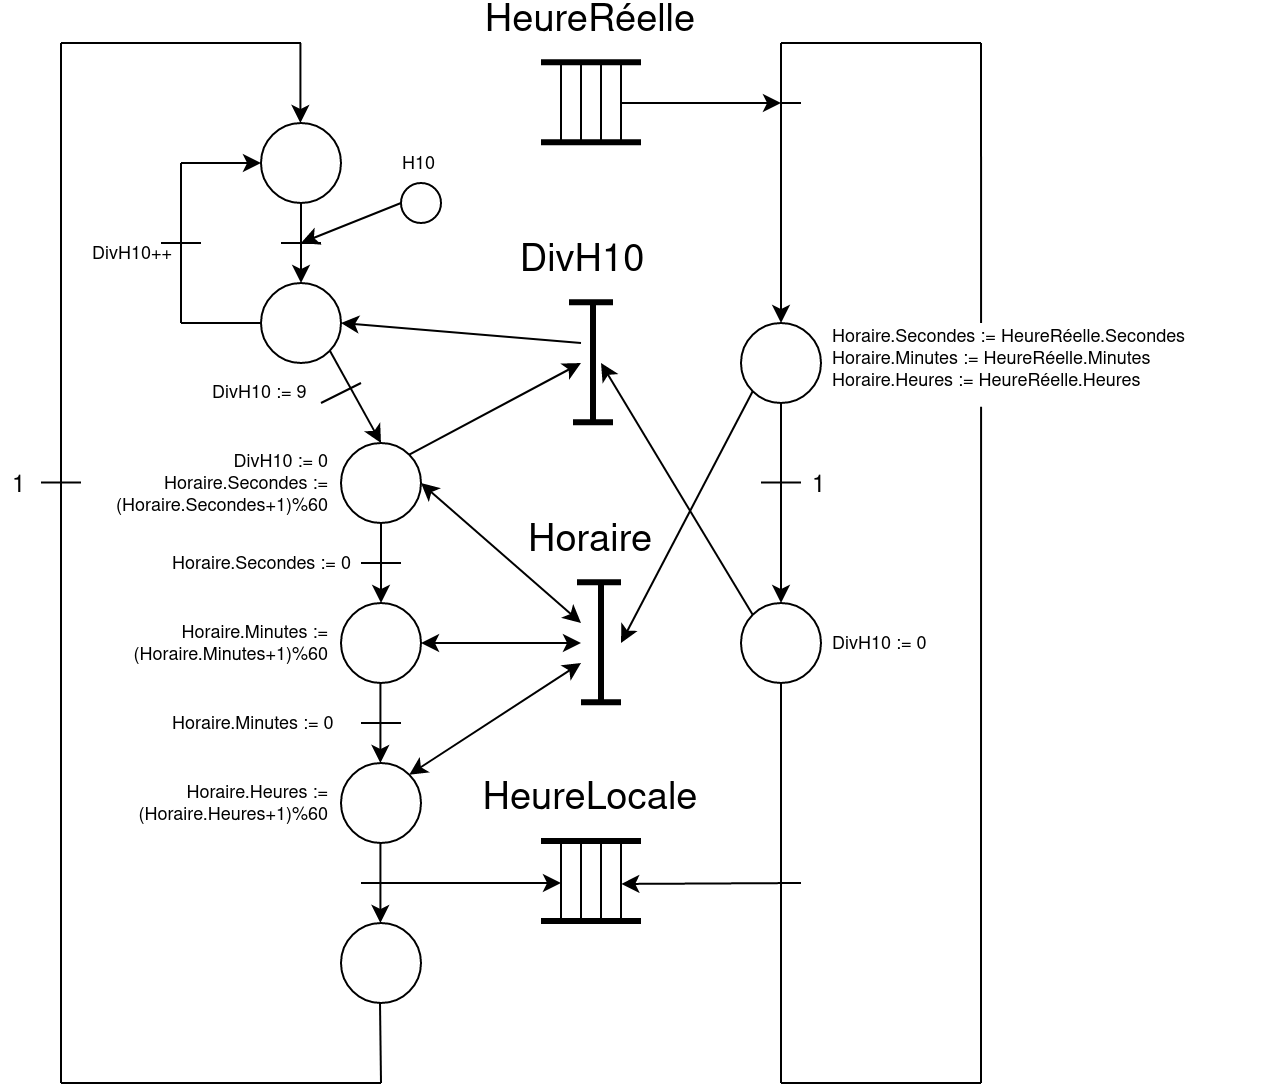
\includegraphics[width=13cm]{photo/reseau_petri}
		\caption{Sortie sur la console}
		\label{fig:reseau_petri}
	\end{figure}
	
	Dans ce réseau on est en présence de deux variables partagées \texttt{Div10} et \texttt{Horaire}. Une question logique à ce poser est : doit on mettre des sémaphores pour éviter des exclusions mutuelles ?\\
	
	La réponse est non car l'environnement est synchrone. Les tâches \texttt{Estime\_Heure} et \texttt{Corrige\_Heure} sont prêtes en même temps puis s'activent en même temps. Cela implique une gestion simple des priorités. C'est pourquoi il est possible d'éviter la mise en place de sémaphore.\\
	
	
	
	\section{Solution classique}
	% Parler de la solution d'implémentation (prépa)
	
	Cette partie vise à mettre en place la solution décrite précédemment. Pour l'implantation sur VxWorks, il est nécessaire d'utiliser les éléments suivants :
	\begin{itemize}
		\item une tâche \texttt{Estime\_Heure};
		\item une tâche \texttt{Estime\_Heure};
		\item une tâche \texttt{Estime\_Heure};
		\item un sémaphore \texttt{H10};
		\item une file de message \texttt{FMHeureLocale};
		\item une file de message \texttt{FMHeureReelle};
		\item une variable partagé \texttt{DivH10};
		\item une variable partagé \texttt{horaire}.		
	\end{itemize}
	
	On précise que la variable \texttt{horaire} est d'un type prédéfini \texttt{type\_heure} qui contient les secondes, les minutes et les heures dans une structure.\\
	
	Pour le bon fonctionnement du programme, il est nécessaire d'attribuer des priorités aux différentes tâches.Dans l’environnement	VxWorks, la tâche de priorité la plus élevée est celle qui dispose du numéro de priorité le plus faible. La tâche de priorité 0 est la plus prioritaire et la tâche de fond est la tâche de priorité 255. On évite d’attribuer les priorités comprises entre 0 et 10, réservée à l’environnement VxWorks. Les priorités suivantes sont affectées aux tâches :
	
	\begin{table}[H]
		\centering
		\begin{tabular}{|c|c|}
			\hline
			Tâche & Priorité \\
			\hline
			\texttt{Estime\_Heure} & 13 \\
			\hline
			\texttt{Corrige\_Heure} & 14 \\
			\hline
			\texttt{Affiche} & 15 \\
			\hline
		\end{tabular}
		\caption{Attribution des priorités aux différentes tâches}
		\label{tab:priorite_taches}
	\end{table}
	
	\subsection{Validation du comportement}
	
	La figure \ref{fig:affichage_comportement_normal} montre la sortie de la console pour une exécution classique du programme.
	
	\begin{figure}[H]
		\centering
		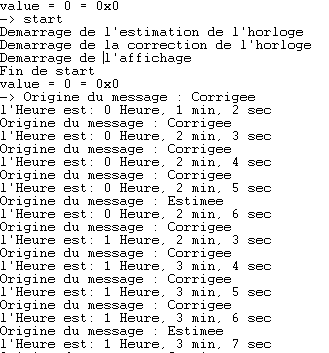
\includegraphics[width=8cm]{photo/affichage_normal/affichage_comportement_normal}
		\caption{Sortie sur la console}
		\label{fig:affichage_comportement_normal}
	\end{figure}
	
	Une fois l'initialisation des tâches effectués dans le \texttt{start}, nous observons un affichage de l'heure provenant des deux tâches. On note que l'heure affiché provient beaucoup plus souvent de \texttt{Corrige\_Heure} que de \texttt{Estime\_Heure}.
	
	
	\begin{figure}[H]
		\centering
		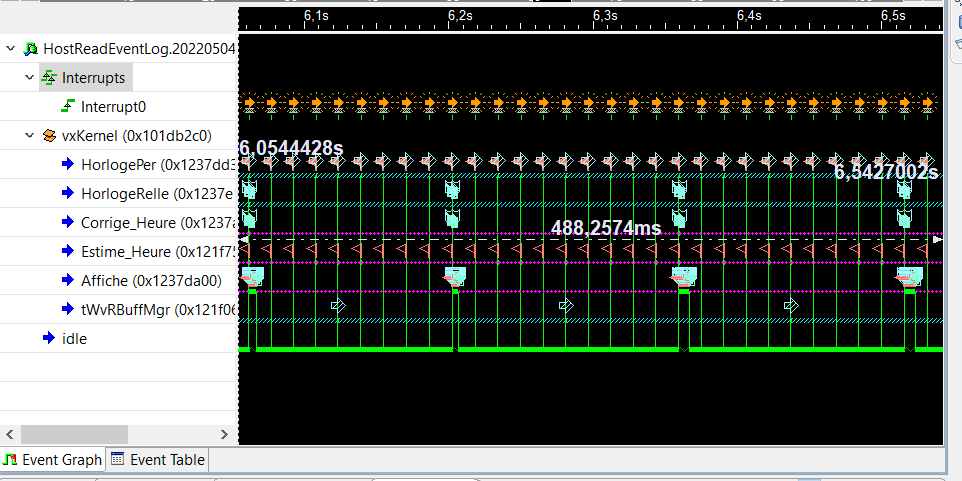
\includegraphics[width=16cm]{photo/affichage_normal/comportement_normal_fois_3}
		\caption{Sortie sur la console}
		\label{fig:affichage_comportement_normal}
	\end{figure}
	
	
	
	\begin{figure}[H]
		\centering
		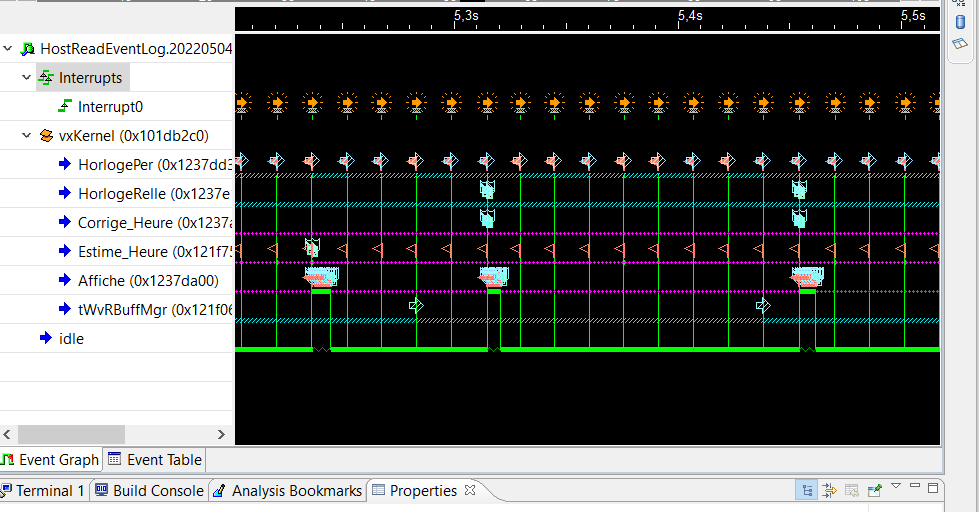
\includegraphics[width=16cm]{photo/affichage_normal/interruption_corrige_heure}
		\caption{Sortie sur la console}
		\label{fig:affichage_comportement_normal}
	\end{figure}
	
	Le code commenté de la solution à un utilisateur pour les priorités ci-dessus est disponible en Annexe 1. La simulation de la situation est lancée et analysée ci-dessous.


	\subsection{Asservissement de la boîte aux lettres}	
	
	\subsection{Différences liées au type de sémaphore}
	
	\section{Variante}

	\section{Conclusion}

	
\end{document}
